\chapter{Approach}\label{chap:approach}

In the field of unsupervised instance detection and segmentation, CutLER~\cite{wang2023cut} gives a strong performance by exploiting a object-centric prior by training on ImageNet~\cite{deng2009imagenet}, as most images contain a single
object in the center of the frame.  Due to its strong instance discrimination abilities, CutLER is the current state-of-the-art method for this task.

In this chapter, we are exploring the limitation of CutLER, looking deeper into the special cases where CutLER fails such as overlapping instances and complex backgrounds. From the drawbacks of CutLER, we propose to train the model without overlapping instances, observing that overlapping instances are one of CutLER's main failure cases. We also investigate the hypothesis that a major reason for the better performance of CutLER is it's object-centric prior. Furthermore, using the gathered information from the observations, we introduce a hypothesis to refine MaskCut masks using CutLER predictions to train the model from scratch to obtain a better evaluation score across a variety of datasets.

\section{Assessing the Limitations of CutLER}
Even though CutLER is the state-of-the-art model for unsupervised instance detection and segmentation, it still has several drawbacks. Mainly We go through some of them in this section.

\subsection{Dependence on Initial Masks}
\begin{figure*}
	\centering
	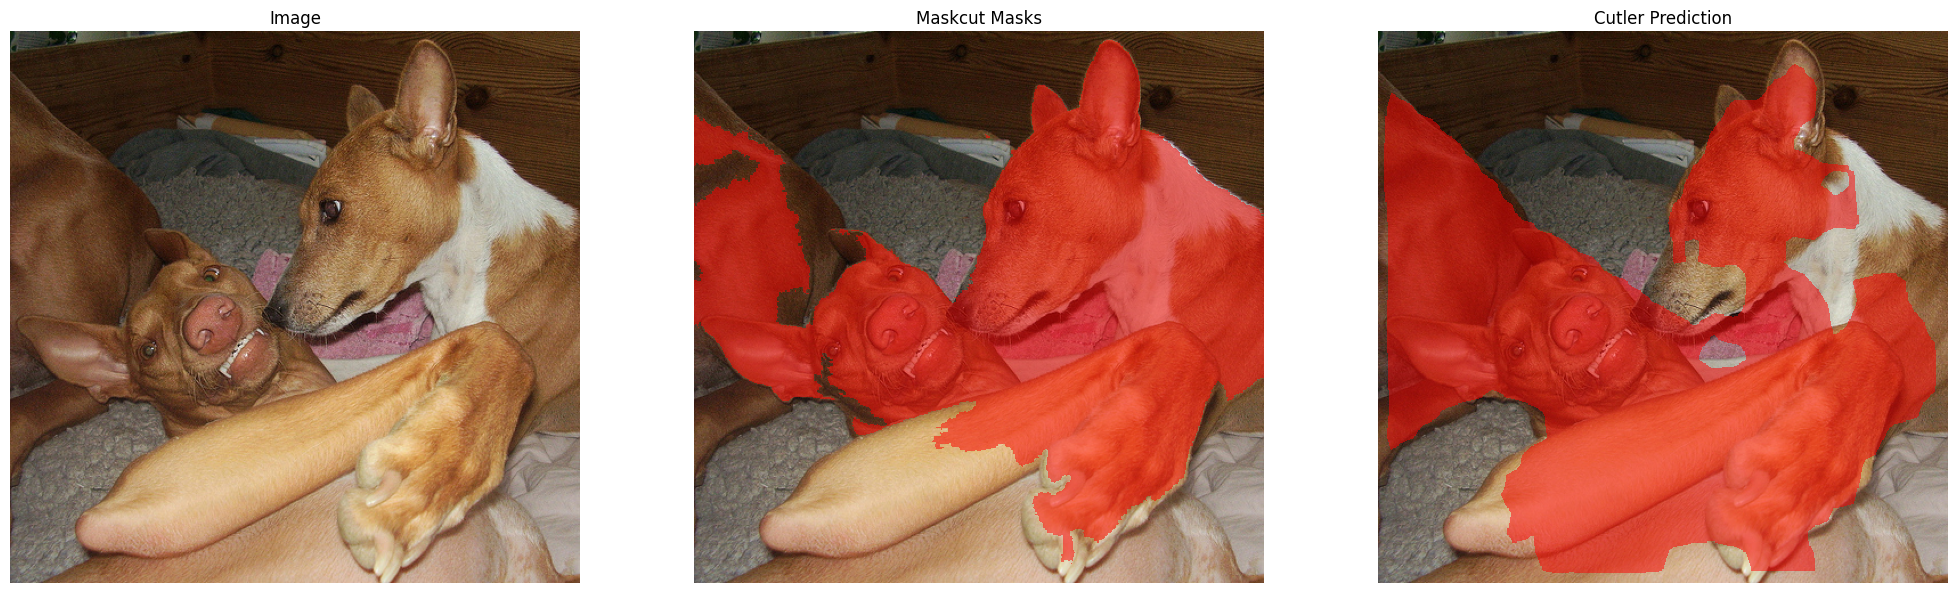
\includegraphics[width=1\textwidth]{Images/main/cutler_problem_3.png}
	\caption[\textbf{Dependence on Initial Masks}]{\textbf{Dependence on initial masks} reflected on the final CutLER prediction}
	\label{fig:intial_mask_dependence}
\end{figure*}

CutLER relies on initial masks provided by MaskCut. If these initial masks are of poor quality, the performance of CutLER may be adversely affected. These pseudo-ground truths often contain inaccuracies due to imperfect initial segmentation, which can arise from factors like complex backgrounds, occlusions, and variations in object appearance. Such imperfections can mislead the model, causing it to learn incorrect features and boundaries, ultimately degrading the quality of instance detection and segmentation. As MaskCut produces the masks based on a hyperparameter N (maximum number of masks generated per image), it also influences the quantity and quality of the pseudo-ground truths.

In challenging scenarios with cluttered backgrounds, occlusions or low-quality images, MaskCut could produce noisy masks as in Fig.~\ref{fig:intial_mask_dependence} which can also affect the quality of CutLER predictions. One common method to filter out good masks is thresholding, which is used in the baseline and our approach during self-training.

%\begin{table}[htbp]
%	\centering
%	\resizebox{1\textwidth}{!}{%
%	\begin{tabular}{c|c|c|c|c|c|c}
%		\toprule
%		\textbf{Methods}               & \textbf{APbox50} & \textbf{APbox} & \textbf{ARbox100} & \textbf{APmask50} & \textbf{APmask} & \textbf{ARmask100} \\ \midrule
%		TokenCut (1 eigenvec.) & 5.2 & 2.6 & 5.0 & 4.9 & 2.0 & 4.4 \\ \midrule
%		TokenCut (3 eigenvec.) & 4.7 & 1.7 & 8.1 & 3.6 & 1.2 & 6.9 \\ \midrule
%		MaskCut (t = 3)        & 6.0 & 2.9 & 8.1 & 4.9 & 2.2 & 6.9 \\ \midrule
%		CutLER                 & 21.9 & 12.3 & 32.7 & 18.9 & 9.7 & 27.1 \\ \midrule
%	\end{tabular}%
%	}
%	\caption{Performance comparison of different methods on box and mask AP/AR metrics.}
%	\label{tab:performance_table}
%\end{table}

To address this issue before self training, in our approach, we filter the MaskCut masks using the CutLER predictions and train from scratch, assuming the learning from scratch using better quality masks could improve the performance of the model. The approach is explained in detail in Section~\ref{section:proposed_method}.

\subsection{Overlapping Instances}
\label{section:overlapping_instances_analysis}
\begin{figure*}
	\centering
	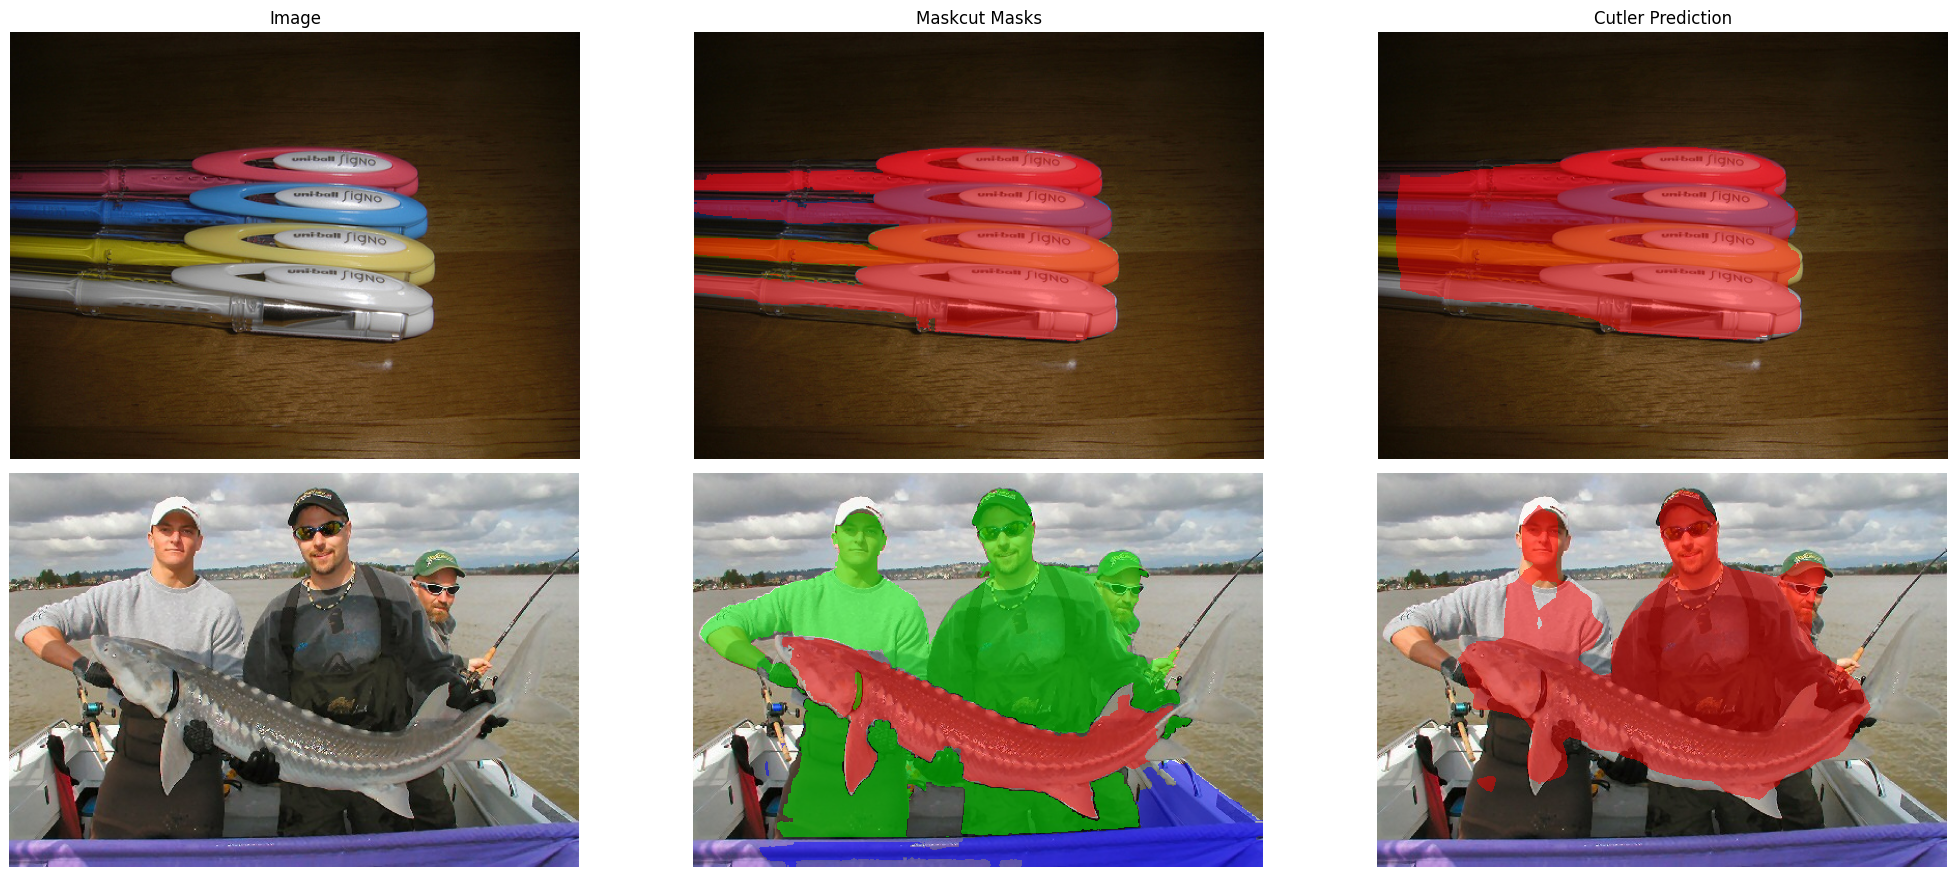
\includegraphics[width=1\textwidth]{Images/main/cutler-prob-overlap.png}
	\caption[\textbf{Cutler's Performance on Images with Overlapping Instances}]{\textbf{Grouping of overlapping instances} in MaskCut and CutLER outputs, which is a common problem in most of the existing unsupervised instance detection methods.}
	\label{fig:cutler_overlapping_instances_eg}
\end{figure*}

Identifying instances using unsupervised instance detection or segmentation methods present significant challenges, especially when instances are closely positioned or overlapping in an image. Overlapping objects often blend together, making it difficult for the model to accurately segment and differentiate them as distinct entities. This lack of explicit supervision complicates the model's ability to learn and generalize the spatial relationships and boundaries between objects.

As illustrated in Fig.~\ref{fig:cutler_overlapping_instances_eg}, in almost all cases of images with overlapping instances, MaskCut and CutLER groups those instances together. MaskCut primarily separates the foreground from the background rather than differentiating between individual instances~\cite{engstler2023understanding}, which is a limitation of this method, which is analyzed in Section~\ref{section:limitations_of_MaskCut}. As a result, in Fig.~\ref{fig:cutler_overlapping_instances_eg}, it can successfully detect the fish but not the group of people as there is an overlap between them. Consequently, in images with overlapping instances, both MaskCut and CutLER generate outputs that are more akin to semantic segmentation than true instance segmentation.

The problem is not exclusive to MaskCut or CutLER, but most of the existing methods~\cite{engstler2023understanding, cond1_support_2, Wang_2022_CVPR} also address this issue. Solving this problem requires devising an algorithm that could use the instance-discriminating representations from DINO and use it to separate the instances. We attempted to address this issue by using Keypoint Correspondences, which is a challenging task. As we could not come up with an graph-cut algorithm that fits problem, it is not a main part of this work. Nevertheless, it can be accessed in the Future Works Section~\ref{section:keypoint-correspondences}.

Another solution to address the grouping of instances would be to provide explicit semantic information of instances during training. It is explored in Wang et al. (2023)~\cite{wang2023cut} by testing with low-shot settings, ie, 2\% and 5\% labeled data, CutLER achieves 5.4\% and 7.3\% higher \(AP_{box}\) than the fully supervised MoCo-v2 with better separation of close and overlapping instances. But as our approach focuses solely on improving the unsupervised instance detection performance, the problem of grouping instances remains unsolved in our approach as well. But we intent to explore the influence of overlapping instances on CutLER training and evaluation which is explained in detail in the next section.


\subsection{Images with Complex Background}
\label{section:images_with complex_backgrounds}
\begin{figure*}
	\centering
	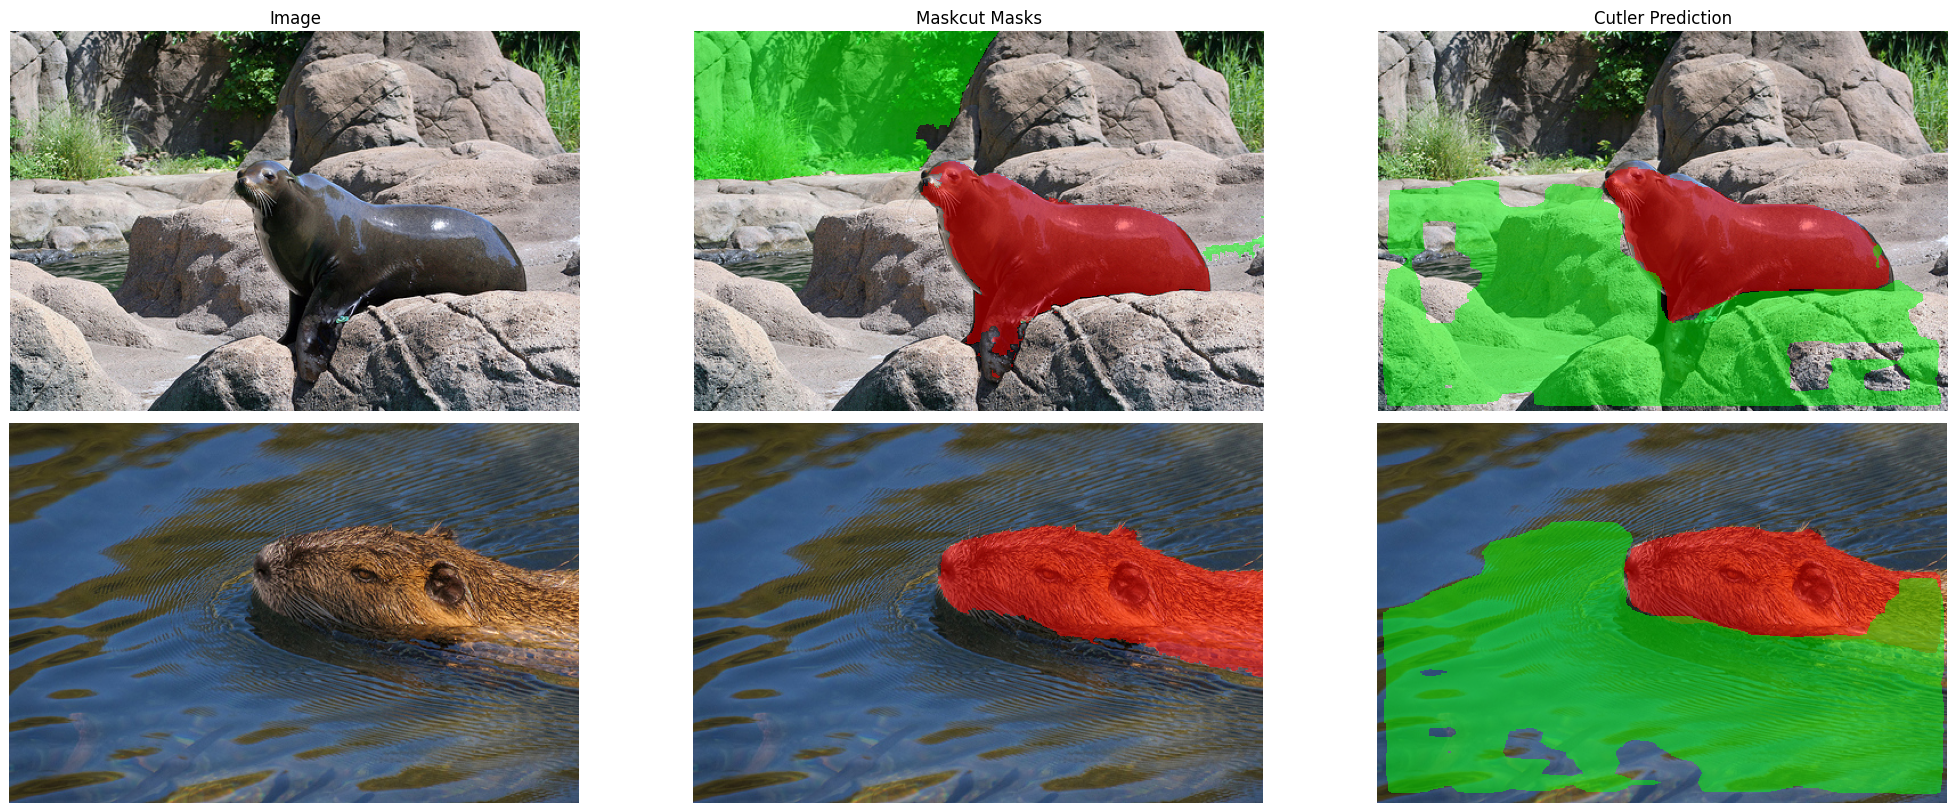
\includegraphics[width=1\textwidth]{Images/main/cutler-prob-noisy-bg.png}
	\caption[\textbf{Cutler's Performance on Images with Complex Background}]{\textbf{Images with complex backgrounds} impacting MaskCut and CutLER outputs, leading to undesired background mask generation}
	\label{fig:cutler_noisy_bg_eg}
\end{figure*}

\begin{figure*}
	\centering
	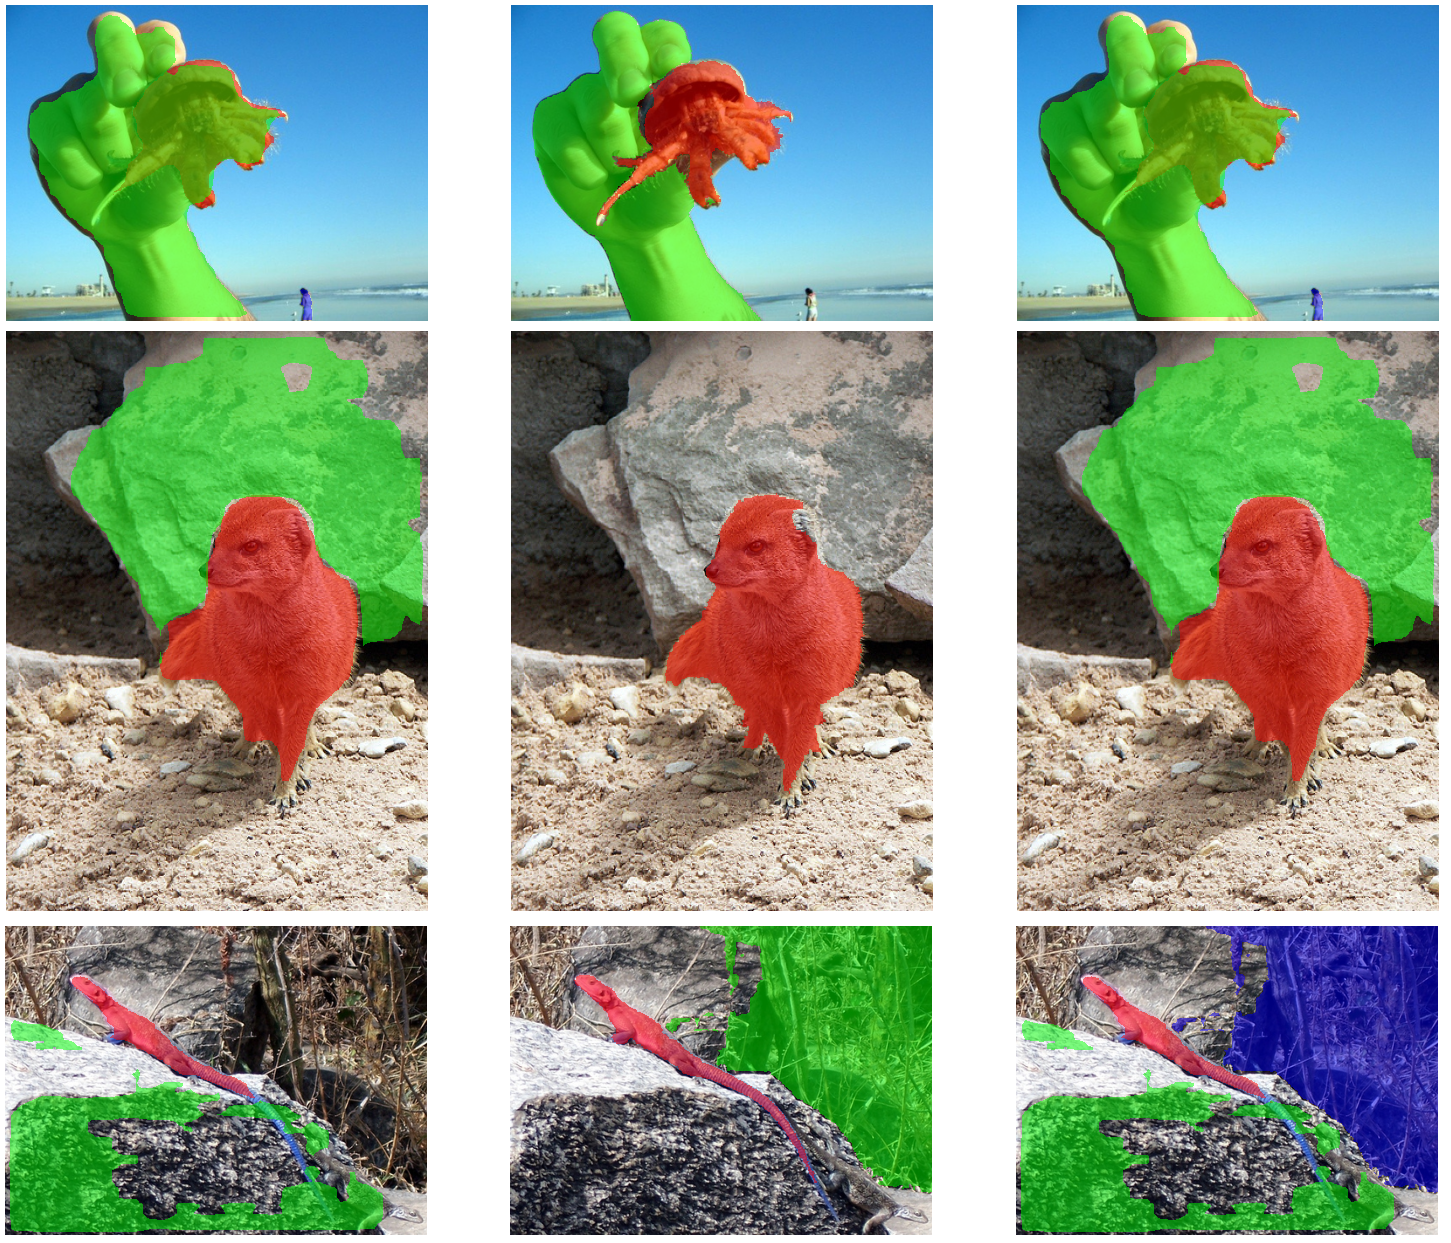
\includegraphics[width=1\textwidth]{Images/main/filtered_mask_problem.png}
	\caption[\textbf{Mask Filtration in Baseline - Qualitative Examples}]{\textbf{Mask Filtration in Baseline - Qualitative Examples} Examples illustrates CutLER prediction masks, MaskCut masks and masks selected by CutLER mask filtration method (left to right)}
	\label{fig:filtered_mask_problem}
\end{figure*}

Even though DINO features are good at providing foreground-background separation, images with complex or unusual backgrounds can possess challenges to this task. In our approach, we intent to address the issue of unwanted masks generated due to complex backgrounds as shown in Fig.~\ref{fig:cutler_noisy_bg_eg}. Such masks can not only be present in the MaskCut masks which act as the pseudo-ground truth for CutLER training, but also in the CutLER predictions itself. As per our observation, the mask filtration strategy used by the baseline doesn't address this issue, which is explained in detail in Section~\ref{sec:baseline_mask_filteration}.

In CutLER, a self-training loop is implemented to iteratively refine the pseudo ground truth masks. We hypothesize that removing undesired background mask before training and self-training phases could improve the performance of the model. We plan to test this hypothesis by modifying the mask filtration algorithm used to refine pseudo-ground truth masks in the baseline method before each self-training loop. This modified algorithm will be used to generate improved MaskCut masks, enabling us to train the model from scratch with better pseudo-ground truth. Our approach addressing this issue is explained in Section~\ref{section:Mask-Filtration}.

\paragraph{Limitation of CutLER Mask Filtration - Qualitative Examples}

Figure~\ref{fig:filtered_mask_problem} illustrates some qualitative examples of how the baseline filters masks for the next round of training. Despite having either good MaskCut mask or CutLER prediction, baseline selects large incorrect MaskCut masks which doesn't overlap much along with CutLER prediction masks, which adversely affect the model performance. We intent to remove these false masks to generate better quality pseudo-ground truths.

\subsection{Suboptimal Use of DINO Features in MaskCut}
\label{section:limitations_of_MaskCut}

\begin{figure*}
	\centering
	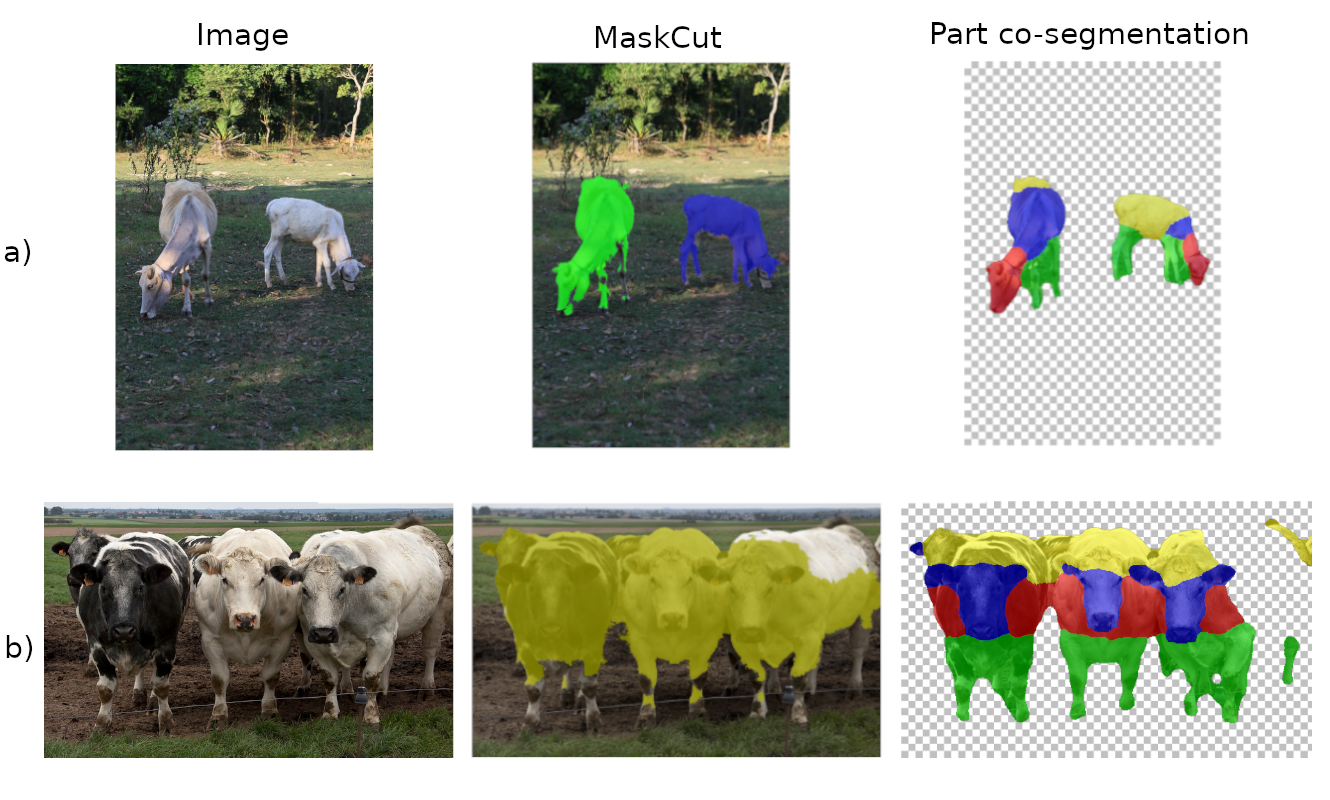
\includegraphics[width=1\textwidth]{Images/main/part-cosegm.png}
	\caption[\textbf{MaskCut vs Part Co-Segmentation Masks}]{\textbf{MaskCut vs Part Co-Segmentation Masks.} Discriminative features that could help differentiate instances are present in DINO features, as evidenced in n-part co-segmentation. But these features are not leveraged by MaskCut. }
	\label{fig:maskcut-instance-indifference}
\end{figure*}

MaskCut is the pseudo-ground truth mask generation method for CutLER. Even though MaskCut proves to be better than other existing methods like TokenCut~\cite{wang2023cut}, it still comes with limitations. 

MaskCut is not effectively making use of the discriminative DINO features that could help differentiate the instances. As it can be observed from Fig.~\ref{fig:maskcut-instance-indifference}, the part co-segmentation map generated by clustering feature maps obtained from the self-attention layers of DINO clearly contains features that could help discriminate these instances. However, MaskCut does not fully utilize these features. Instead, it operates more on a coarse level by segmenting the image into foreground and background regions.

MaskCut also comes with a fixed hyperparameter N, which determines the maximum number of masks to be produced per image, regardless of the actual number of distinct instances present. This constraint limits its flexibility and effectiveness, especially in complex scenes with multiple instances. As a result, MaskCut often under-segment instances even though the instance discriminative features are provided by DINO.

\section{Proposed Approaches}

\subsection{Approach to Estimate the Impact of Overlapping Instances}
\label{section:analysis_ol_instancs}

Based on the observation that MaskCut often groups overlapping instances into a single mask from Section~\ref{section:overlapping_instances_analysis}, we hypothesize that training CutLER on ImageNet images without overlapping instances may improve performance compared to training on all images. This approach could reduce the number of inaccurate masks (removing grouped instance masks), improving the overall quality of pseudo-ground truth masks. Additionally, we aim to explore whether a model trained exclusively on non-overlapping instances can enhance detection of individual instances in images where overlaps occur.

For the sake of completeness and to observe whether there is any relative improvement or loss, we compare three approaches of training CutLER. 

\begin{enumerate}
	\item Using all images of ImageNet (Same as the baseline)
	\item Using images without any overlapping instances 
	\item Only using images with overlapping instances
\end{enumerate}

We expect that the model trained without overlapping instances will outperform the baseline, while the model trained exclusively on images with overlapping instances will likely underperform compared to the baseline. Splitting the evaluation dataset according to these three approaches should also reveal a similar performance pattern. Our hypotheses is supported by the positive results from the experiments in Section~\ref{section:overlapping-results}.

To test the hypothesis, we make use of ground truth bounding box annotations provided by ImageNet and the images with an overlap (IoU) of \(\tau > \text{0.1}\) is taken as the criteria to filter images for approach 2 and 3. As ImageNet contains mostly object-centric single instance images, the third approach (only using images with overlapping instances) would have significantly less number of training images compared to the other two approaches. Specifically, Approach 3 utilizes 6\% of the annotated ImageNet dataset, while Approach 2 uses the remaining 94\%. Given the significantly smaller training sample size in Approach 3, a fair comparison isn't possible. Therefore, we focus on Approach 2 for comparison with the baseline.

Through this approach, we expect to observe an improvement by using less training data. But using this method in unsupervised fashion is rather difficult. Due to the grouping of nearby instances, the process of filtering images with overlapping instance is extremely challenging. Hence these tests are carried out using bounding box labels of ImageNet. However, the approach gives insights on the influence of overlapping instances in training that can be useful for future research.

\subsection{Approach to Estimate the Impact of Object-Centric Instances}
\label{section:analysis_oc_instancs}
To support our hypothesis that an object-centric prior is a key contributor to CutLER's state-of-the-art performance, we propose that filtering out non-object-centric images from the training dataset could further enhance its effectiveness. Recent research has highlighted the significant role that object-centric images play in model performance~\cite{engstler2023understanding, Gasparim_2021}.

Object-centricity is hard to define. As we couldn't find a standard way to define object-centicity for our research~\cite{Russakovsky, Gasparim_2021}, we defined two simple hyperparameters to filter object-centric images.

\begin{itemize}
	\item \textbf{Area Threshold} : Minimum area ratio of bounding box to image
	\item \textbf{Center Threshold} : Maximum distance ratio from the image center to bounding box center to the image diagonal.
\end{itemize}

We set Area Threshold to 0.1 and Center Threshold to 0.2. That is, if bounding box has size less than 10\% of the size of the image or the distance between image center and bounding box center is more than 20\% of image's diagonal length, that image will be rejected from the training set.

Like in the previous section, to test the hypothesis, we make use of ground truth bounding box annotations provided by ImageNet. We are only using single instance images as object-centric images can contain overlapping instances as well. Due to the filtration process, we only use 77\% images of annotated ImageNet dataset, that is only 30\% of total ImageNet images. Even with this much less data, we expect to observe a competitive result compared to the baseline. 


\subsection{Approach for Mask Filtration}
\label{section:Mask-Filtration}
Considering the problems with complex backgrounds and limitations of CutLER Mask Filtration method in Section~\ref{section:images_with complex_backgrounds}, We propose a new mask filtration method to address these issues. In this section, we also provide a detailed explanation of the baseline (CutLER) mask filtration method, making it easier to understand the improvements offered by our approach.

\subsubsection{CutLER Mask Filtration Method}
\label{sec:baseline_mask_filteration}
To improve clarity and facilitate comparison with the proposed method, we break down the CutLER training process into two distinct phases: initial training and self-training, as illustrated in the Fig.~\ref{fig:baseline_training}.

\begin{figure*}
	\centering
	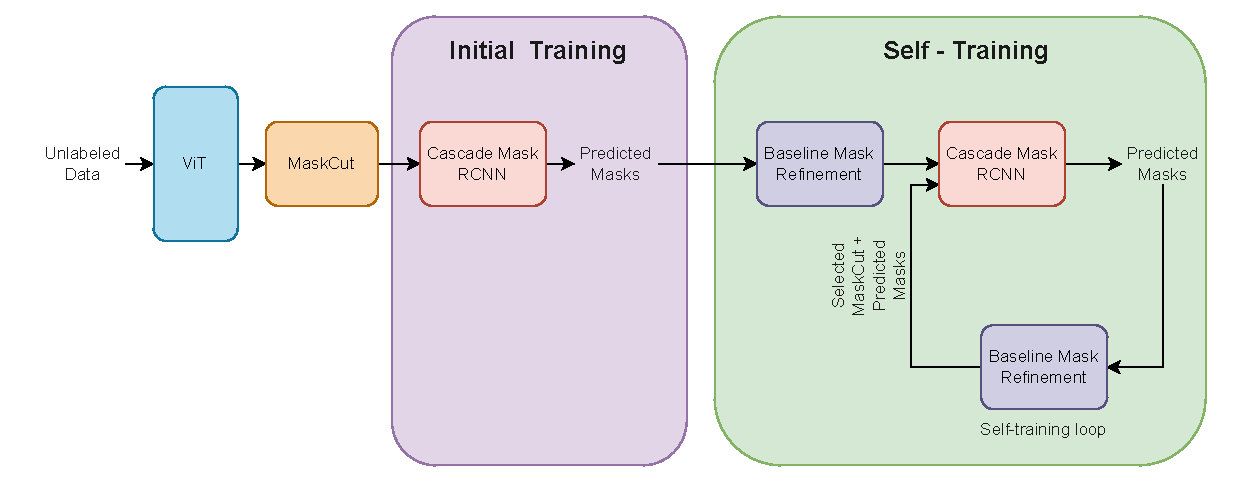
\includegraphics[width=1\textwidth]{Images/main/baseline_approach.pdf}
	\caption[\textbf{Baseline Training Pipeline}]{\textbf{Baseline training pipeline} with repeated mask filtration and self-training}
	\label{fig:baseline_training}
\end{figure*}

\paragraph{Initial Training}
Initially, the detector (Cascade Mask RCNN) trained with  ImageNet dataset using MaskCut masks as pseudo-ground truth for 160K iterations with Copy-Paste augmentations and DropLoss. As illustrated in Fig.~\ref{fig:baseline_training}, after the initial training, the trained model predicts masks for each image in ImageNet dataset (30 masks per image) using the trained model. Out of the 30 predicted masks, high-quality ones are filtered by applying a confidence score threshold of 0.7 and passed onto the mask filtration pipeline. 

\begin{figure*}
	\centering
	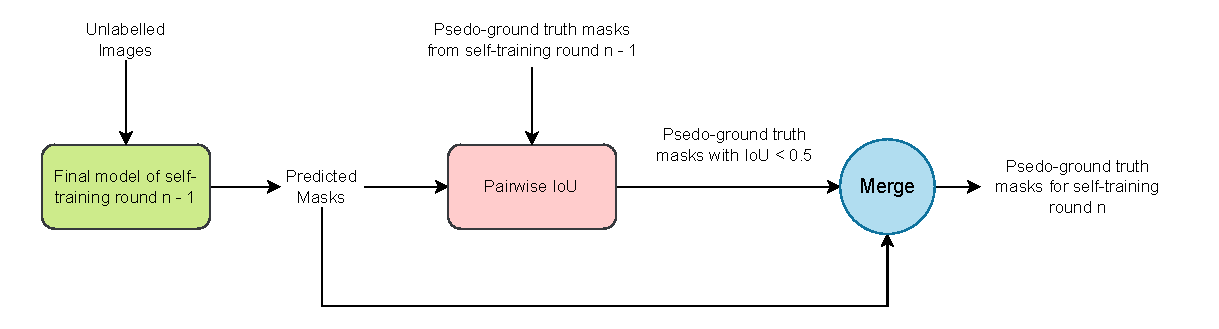
\includegraphics[width=1\textwidth]{Images/main/baseline_mask_filtration.pdf}
	\caption[\textbf{Mask Filtration Method in Baseline}]{\textbf{Mask Filtration in Baseline} before each self-training loop}
	\label{fig:baseline_mask_filtration}
\end{figure*}


\paragraph{Mask Filtration and Self-Training}
Baseline mask filtration process is illustrated in Fig.~\ref{fig:baseline_mask_filtration}.  Pairwise IoU is calculated between the selected predicted masks and MaskCut masks. For mask pairs with an IoU below 0.5, the corresponding MaskCut masks are included, along with all selected predicted masks, to form the pseudo-ground truths for the next self-training stage. Intuitively, MaskCut masks that have less than 50\% overlap with the selected predicted masks are included alongside the CutLER masks to form pseudo-ground truths for next self-training round. 

The goal is to retain as many non-overlapping masks as possible. However, always including masks that don't overlap with CutLER prediction masks can introduce irrelevant or unwanted masks into the pseudo-ground truth. This can affect the performance of the model.

For further self-training loops, the same procedure repeats, except that instead of MaskCut masks, pseudo-ground truth masks of the last round are used to compare with the predicted CutLER masks. Performance of the model claims to have improved upto 3 self-training loops by the authors. We will be running 2 self-training loops for both the baseline and proposed method in our experiments.


\subsubsection{Proposed Mask Filtering Method}
\label{section:proposed_method}

\begin{figure*}
	\centering
	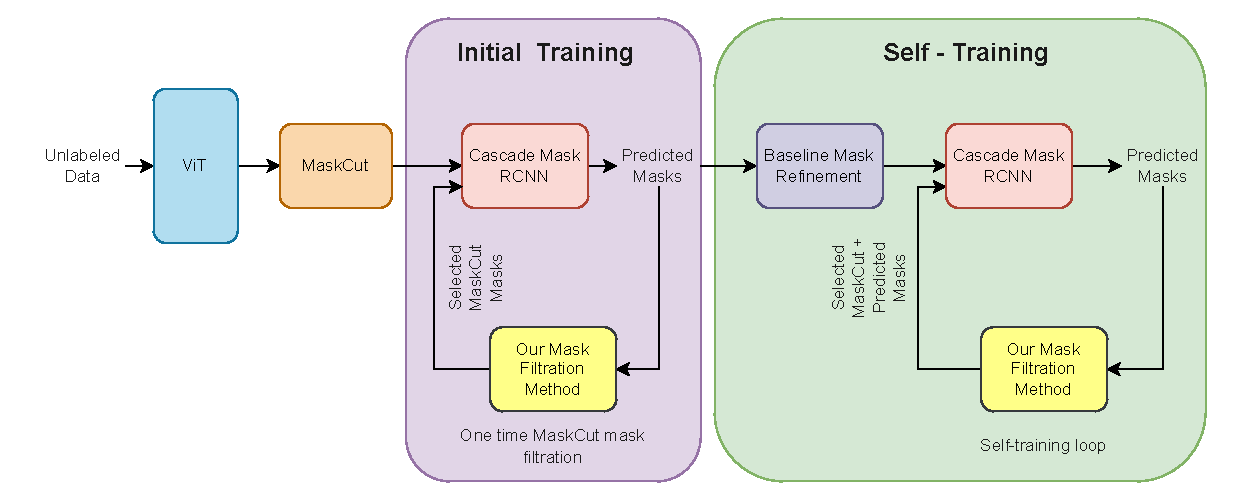
\includegraphics[width=1\textwidth]{Images/main/proposed_method_last.pdf}
	\caption[\textbf{Proposed Training Pipeline 1}]{\textbf{Proposed Training Pipeline 1} featuring a one-time proposed MaskCut mask filtration followed by multiple self-training loops with our mask filtration method.}
	\label{fig:proposed_training}
\end{figure*}
Emphasizing quality over quantity, we introduce an improved approach for mask filtration. Noting that the current mask filtration method in CutLER tends to include unwanted background masks in its pseudo ground truths, we propose to enhance the process by removing ambiguous masks from the ground truth instead of retaining them. This adjustment aims to improve the overall quality and reliability of the pseudo ground truths, leading to better model performance.
´
\paragraph{Initial Training}
\begin{figure*}
	\centering
	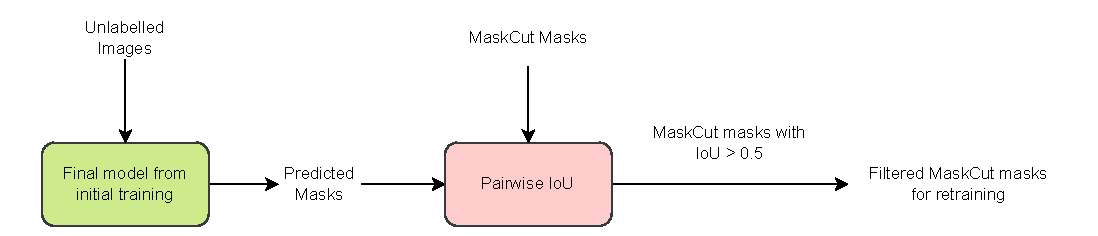
\includegraphics[width=1\textwidth]{Images/main/our_mask_filtration_1.pdf}
	\caption[\textbf{Mask Filtration in Proposed Method}]{\textbf{Mask Filtration in Our Method}, used to filter MaskCut masks after the initial training.}
	\label{fig:our_mask_filtration}
\end{figure*}

As illustrated in Fig.~\ref{fig:proposed_training}, we train the detector for 160K iterations using Copy-Paste augmentations and DropLoss identical to the baseline. After which we introduce an additional step to refine MaskCut masks. This refinement involves preserving only high-certainty masks by comparing them against CutLER predictions.

\paragraph{Proposed Mask Filtration and Retraining}
Proposed mask filtration method is illustrated in Fig.~\ref{fig:our_mask_filtration}. After the first training phase, like in the baseline, high-quality predicted masks are filtered by applying a confidence score threshold of 0.7.  Instead of creating the new pseudo-ground truth by selecting masks from both MaskCut masks and CutLER prediction masks, we focus solely on filtering MaskCut masks. Rather than selecting MaskCut masks corresponding to mask pairs with an IoU < 0.5 from the batch IoU matrix, we choose MaskCut masks that correspond to mask pairs with an IoU > 0.5. 

The idea is to filter highly certain MaskCut masks and discard possible incorrect masks. This selected MaskCut masks are treated as the new pseudo-ground truth and we train from scratch for 160K iterations with Copy-Paste augmentations and DropLoss. We are effectively repeating the same initial training process, but with better masks. With the filtered high quality masks in hand, we expect to achieve a better performance. 

It’s important to note that if no masks are selected for an image, that image is removed from the training set, resulting in a smaller dataset and reducing the training time (Around 130K images are dropped from ImageNet during this stage). This approach effectively eliminates potentially unwanted masks from the pseudo-ground truth, possibly providing more accurate mask predictions.

\paragraph{Further Mask Filtration and Self-Training}
\label{section:proposed_mask_filtration_self_training}
\begin{figure*}
	\centering
	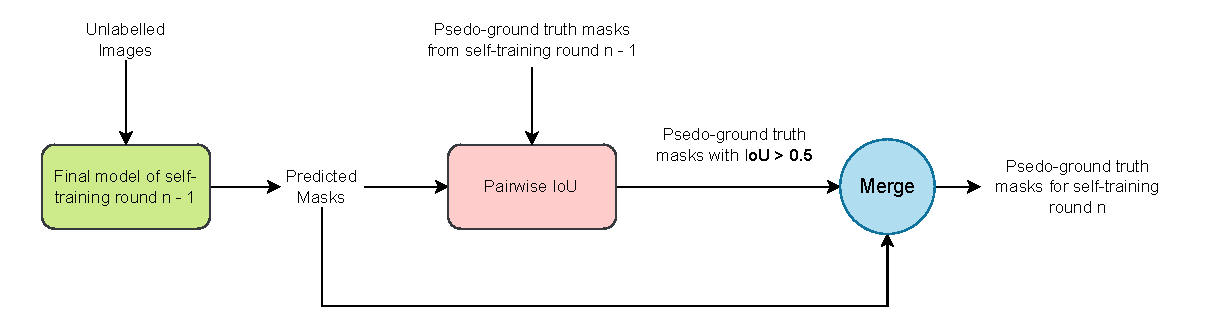
\includegraphics[width=1\textwidth]{Images/main/our_filtration_self_training.pdf}
	\caption[\textbf{Mask Filtration in Proposed Method During Self-Training}]{\textbf{Mask Filtration in Proposed Method}, used to filter masks during self-training.}
	\label{fig:our_mask_filtration_self_training}
\end{figure*}


 For self-training, we follow training pipeline of the baseline, training for 80K iterations are without using DropLoss. We use our mask filtration method illustrated in Fig~\ref{fig:our_mask_filtration_self_training} to filter masks between self-training rounds. 
 
\paragraph{Using Our Mask Filtration Strategy for Self-Training}
\label{para:our_mask_filtration}
The only modification to the baseline approach in self-training loop is selecting pseudo-ground truth masks with IoU > 0.5 with predicted masks, rather than those with IoU < 0.5. This way, we always retain masks with high certainty. 

But this also restricts the exploration. Limiting pseudo-ground truth labels to only high-confidence masks could constrain improvements in the self-training round. The experiments carries out using our mask filtration method in self-training can be accessed in Section~\ref{section:mask_refinement_experiment}.
 
\paragraph{Combination of Mask Filtration Strategies}
\begin{figure*}
	\centering
	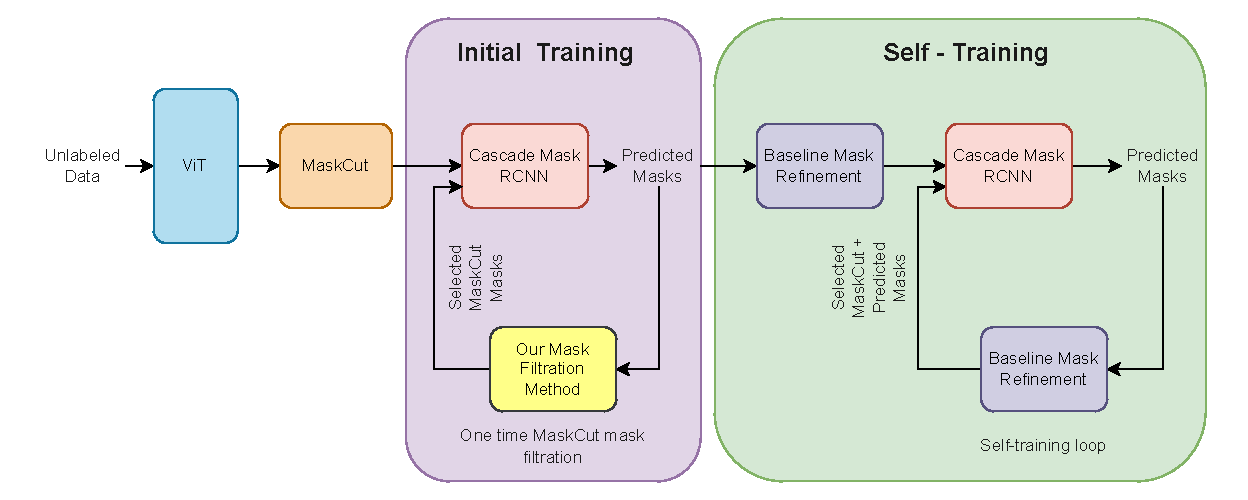
\includegraphics[width=1\textwidth]{Images/main/our_approach.pdf}
	\caption[\textbf{Proposed Training Pipeline 2}]{\textbf{Proposed Training Pipeline 2} featuring a one-time proposed MaskCut mask filtration followed by multiple self-training loops with CutLER mask filtration method.}
	\label{fig:proposed_training_new}
\end{figure*}

Considering the possible issues of employing our mask filtration method in the self-training loop as mentioned in the last section such as limiting exploration and having few masks compared to the baseline, we also intent to test the combination of both. 

As our proposed mask filtration method is rather conservative, we propose to use masks generated using our mask filtration method for initial training and baseline mask filtration strategy for self-training. This way, we can provide more refined masks for initial training and still encourage exploration during self-training. 

The training pipeline is illustrated in Fig.~\ref{fig:proposed_training_new}. The only change is replacing our mask filtration method with the CutLER mask filtration method in the self-training part. This method showed the best performance among the proposed unsupervised approaches, with detailed experimental results provided in Section~\ref{section:mask_refinement_experiment}.

 
\paragraph{Recall Reduction Concerns}
By utilizing a smaller number of more accurate masks, we anticipate an improvement in precision. However, there may be a slight decrease in recall if the reduced number of masks does not sufficiently cover all ground truth instances. But our experiments indicate that this change is negligibly small. Detailed results and analysis on this can be found in the Section~\ref{section:persistant_recall}.


 %This intuition is validated by our experiments in Section <secno>.

%We use baseline filtration method during self-training. As we already have finer masks, refining further might lead to over-fitting. Limiting pseudo-ground truth labels to only high-confidence masks (like in our filtration method) could constrain improvements in the self-training round. Hence baseline filtration


%\begin{figure*}[h]
%	\centering
%	\begin{subfigure}[b]{0.47\textwidth}
%		\centering
%		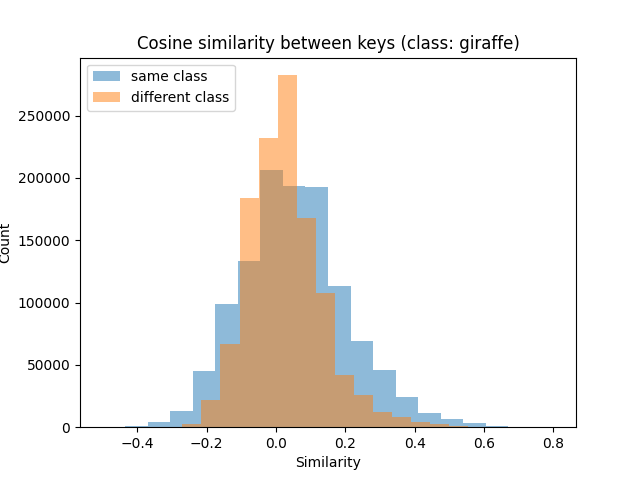
\includegraphics[width=\textwidth]{Images/same_vs_diff_class/plot_giraffe_cosine.png}
%		\caption{Cosine similarity}
%	\end{subfigure}
%	\quad
%	\begin{subfigure}[b]{0.47\textwidth}  
%		\centering 
%		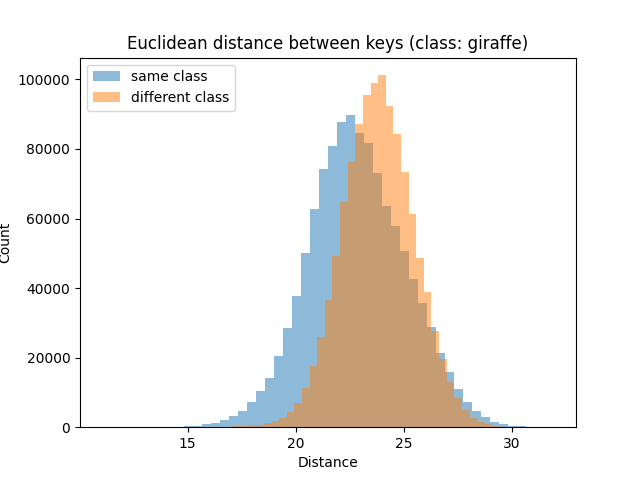
\includegraphics[width=\textwidth]{Images/same_vs_diff_class/plot_giraffe_euc.png}
%		\caption{Euclidean}
%	\end{subfigure}
%	\caption[\textbf{Comparison of keys of images of same and different classes}]{\textbf{Comparison of keys of images of same and different classes}. Shows the pattern of similarity scores and distance measure when comparing keys of same and different classes. Y axis shows number of images compared }
%	\label{fig:same_vs_diff}
%\end{figure*}